\chapter{Theoretical Background}
\label{chap:Theory}
\section{Jet Algorithms}
\label{sec:jet_algos}
\cleardoublepage

\begin{comment}
Predictions at NLO accuracy in pQCD are computed with the \NLOJETPP
program version~4.1.3~\cite{Nagy:2001fj,Nagy:2003tz}. The results are
provided within the framework of \fastNLO
version~2.3~\cite{Britzger:2012bs} for use within fits. The
renormalization and factorization scales \mur and \muf are chosen
equal to \httwo. PDF sets at NLO available for a series of different
assumptions on \alpsmz via the \LHAPDFS package~\cite{Buckley:2014ana}
are listed in Table~\ref{tab:chap2:nlopdfsets}. All sets employ a
variable-flavour number scheme with at most five or six flavours apart
from the ABM11 PDFs, which use a fixed-flavour number scheme with
$\NF=5$.

Out of these eight PDF sets the following three will not be considered
further:
%
\begin{itemize}
\item At NLO, predictions based on ABM11 do not describe LHC jet data
  at small jet rapidity, cf.\ Refs.~\cite{Aad:2013lpa, Aad:2014vwa,
    CMS:2014mna, Khachatryan:2015luy}.
\item The HERAPDF2.0 set exclusively fits HERA DIS data with only weak
  constraints on the gluon PDF\@.
\item The range in values available for \alpsmz is too limited for the
  NNPDF3.0 set.
\end{itemize}
%

PDF uncertainties are evaluated according to the prescriptions given
for each PDF set. Uncertainties on \alpsmz are not considered, since
this value is later on determined from a fit to the data. The PDF
uncertainty as derived with the CT10 PDF set ranges from 2\% to 30\%
for inclusive 2- and 3-jet cross sections and from 2\% to 7\% for \ratio.

\begin{table}[htbp]
  \centering
  \caption{NLO PDF sets available via \LHAPDFS for comparisons to data with
    various assumptions on the value of \alpsmz. Sets existing already in
    LHC Run~1 (upper rows) and newer sets for Run~2 (lower rows) are
    listed together with the corresponding number of flavours \NF, the
    assumed masses $M_t$ and $M_Z$ of the top quark and the $Z$ boson,
    respectively, the default values of \alpsmz, and the range in \alpsmz
    variation available for fits.  A~$^*$ behind the \alpsmz values
    signifies that the parameter was fixed, not fitted.}
  \label{tab:chap2:nlopdfsets}
  \begin{tabular}{llccllc}
    \hline\hline
    Base set & Refs. & \NF & $M_t$ (\GeVns{}) &
    $M_Z$ (\GeVns{}) &\alpsmz & \alpsmz range\rbthm\\
    \hline
    % LHC Run 1
    ABM11     & \cite{Alekhin:2012ig}
    &       5   & 180       & 91.174  & $0.1180$   & 0.110--0.130\rbtrr\\
    CT10      & \cite{Lai:2010vv}
    & ${\leq}5$ & 172       & 91.188  & $0.1180^*$ & 0.112--0.127\rbtrr\\
    MSTW2008  & \cite{Martin:2009iq,Martin:2009bu}
    & ${\leq}5$ & $10^{10}$ & 91.1876 & $0.1202$   & 0.110--0.130\rbtrr\\
    NNPDF2.3  & \cite{Ball:2012cx}
    & ${\leq}6$ & 175       & 91.1876 & $0.1180^*$ & 0.114--0.124\rbtrr\\\hline
    % LHC Run 2
    CT14      & \cite{Dulat:2015mca}
    & ${\leq}5$ & 172       & 91.1876 & $0.1180^*$ & 0.113--0.123\rbtrr\\
    HERAPDF2.0& \cite{Abramowicz:2015mha}
    & ${\leq}5$ & 173       & 91.1876 & $0.1180^*$ & 0.110--0.130\rbtrr\\
    MMHT2014  & \cite{Harland-Lang:2014zoa}
    & ${\leq}5$ & $10^{10}$ & 91.1876 & $0.1180^*$ & 0.108--0.128\rbtrr\\
    NNPDF3.0  & \cite{Ball:2014uwa}
    & ${\leq}5$ & 173       & 91.2    & $0.1180^*$ & 0.115--0.121\rbtrr\\
    \hline\hline
  \end{tabular}
\end{table}

The uncertainty related to unknown higher orders of the perturbative
series is evaluated with the conventional recipe of varying the
default scale \httwo chosen for \mur and \muf independently in the
following six combinations: (\mur/\httwo, \muf/\httwo) = (1/2,1/2),
(1/2,1), (1,1/2), (1,2), (2,1) and (2,2). The maximal upwards and
downwards deviations in cross section from the central prediction are
taken as scale uncertainty. This uncertainty ranges for inclusive
2-jet events from 5\% to 13\%, for inclusive 3-jet events from 11\%
to 17\% and for their ratio \ratio from 6\% to 8\%.

The computation of the NLO predictions with \NLOJETPP is also subject
to statistical fluctuations from the numerical integrations.  For the
inclusive 2-jet event cross sections this uncertainty is smaller than
about one per mille, while for the inclusive 3-jet event cross section
it amounts to 1--9 per mille.

Higher order effects of electroweak origin affect jet cross sections at large
jet \pt. These electroweak (EWK) corrections have been calculated for
the inclusive 1-jet and 2-jet case, cf.\ Ref.~\cite{Dittmaier:2012kx},
but are not yet known for 3-jet production. Therefore, they are
considered for the 2-jet events, while for the 3-jet event cross
section and for the ratio they have been neglected.

The impact of nonperturbative (NP) effects, \ie from multiple-parton
interactions (MPI) and hadronization, are evaluated by using samples
obtained from different MC event generators with a simulation of
parton-shower and underlying-event (UE) contributions. The leading
order (LO) MC event generators \HERWIGPP~\cite{Bahr:2008pv} with the
default tune of version~2.3 and \PYTHIAS~\cite{Sjostrand:2006za} with
tune \Ztwostar are considered, and the dijet NLO prediction from
\POWHEG~\cite{Nason:2004rx, Frixione:2007vw, Alioli:2010xa} interfaced
to \PYTHIAE with tune CUETS1~\cite{Khachatryan:2015pea} for full event
generation. The cross section ratios between a nominal event
generation and a sample without hadronization and MPI effects are
taken as correction separately for inclusive 2-, and 3-jet events, and
as their ratio for \ratio. This ratio is fitted by a power-law
function. The differences in the correction factors obtained from the
various MC event generators are assigned as an uncertainty. The
central correction factors $C^{\mathrm{\tiny{NP}}}$ are determined by
the centre of the envelope which covers all predictions and half of
the spread is taken as the uncertainty.

\begin{figure}[h]
  \hftwo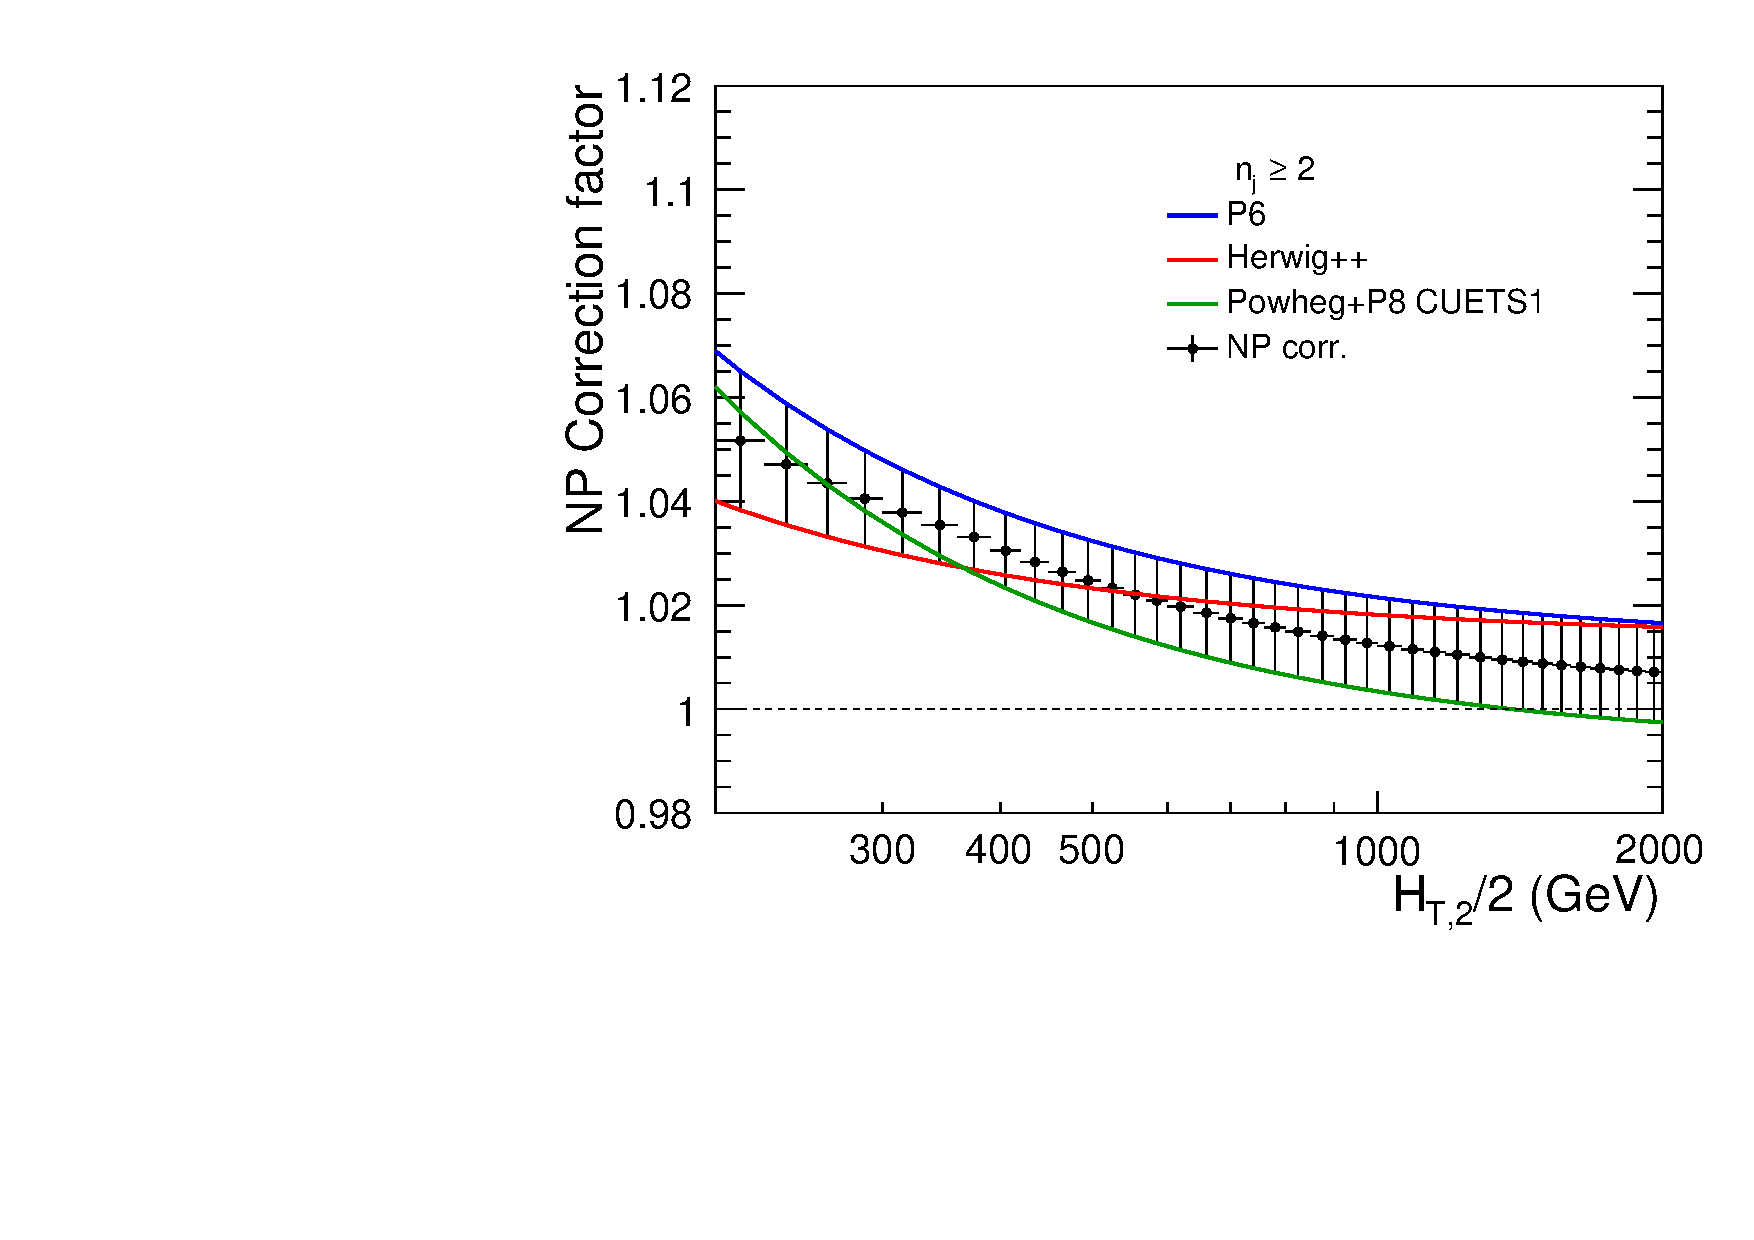
\includegraphics[width=0.5\textwidth]{Plots_PAS/Final_NP_Corr_2.pdf}\hftwo%
  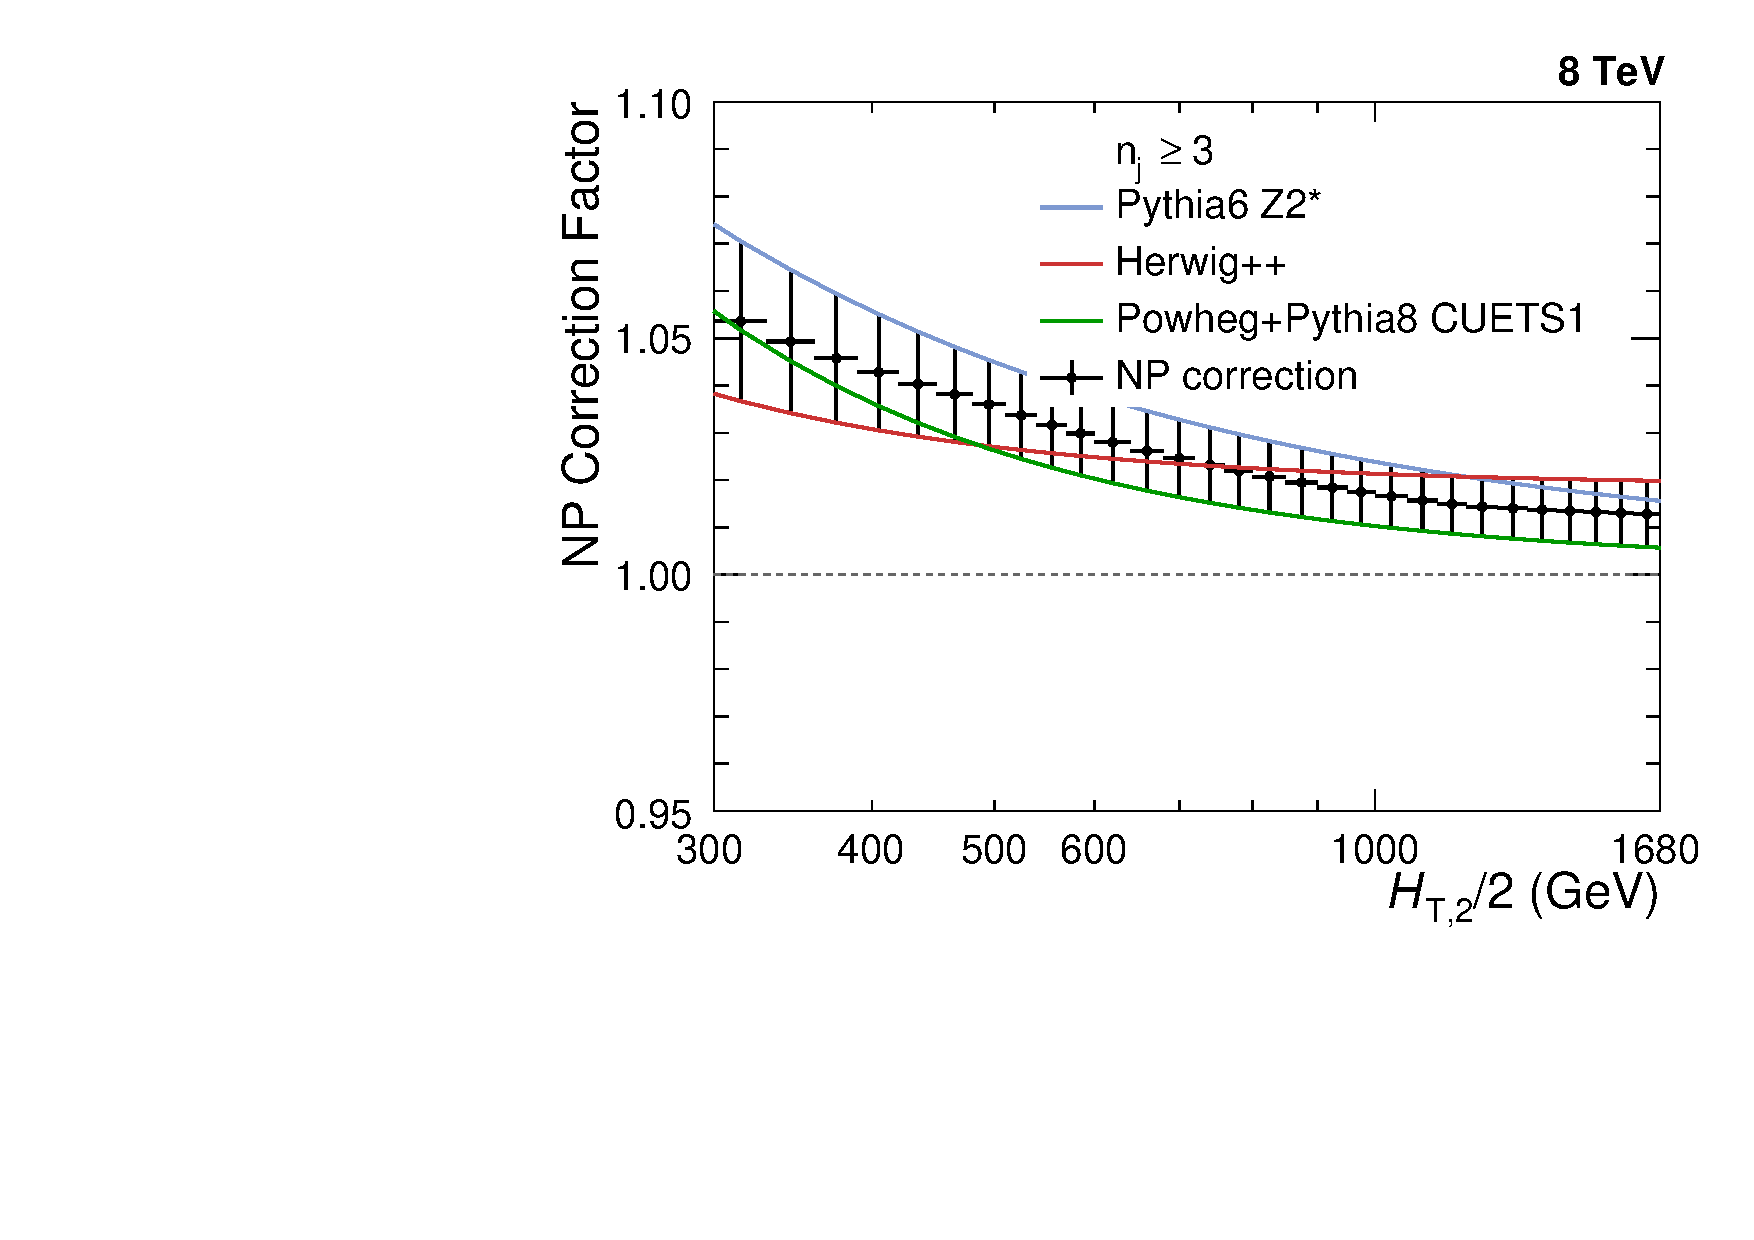
\includegraphics[width=0.5\textwidth]{Plots_PAS/Final_NP_Corr_3.pdf}\hftwo\\
  \hftwo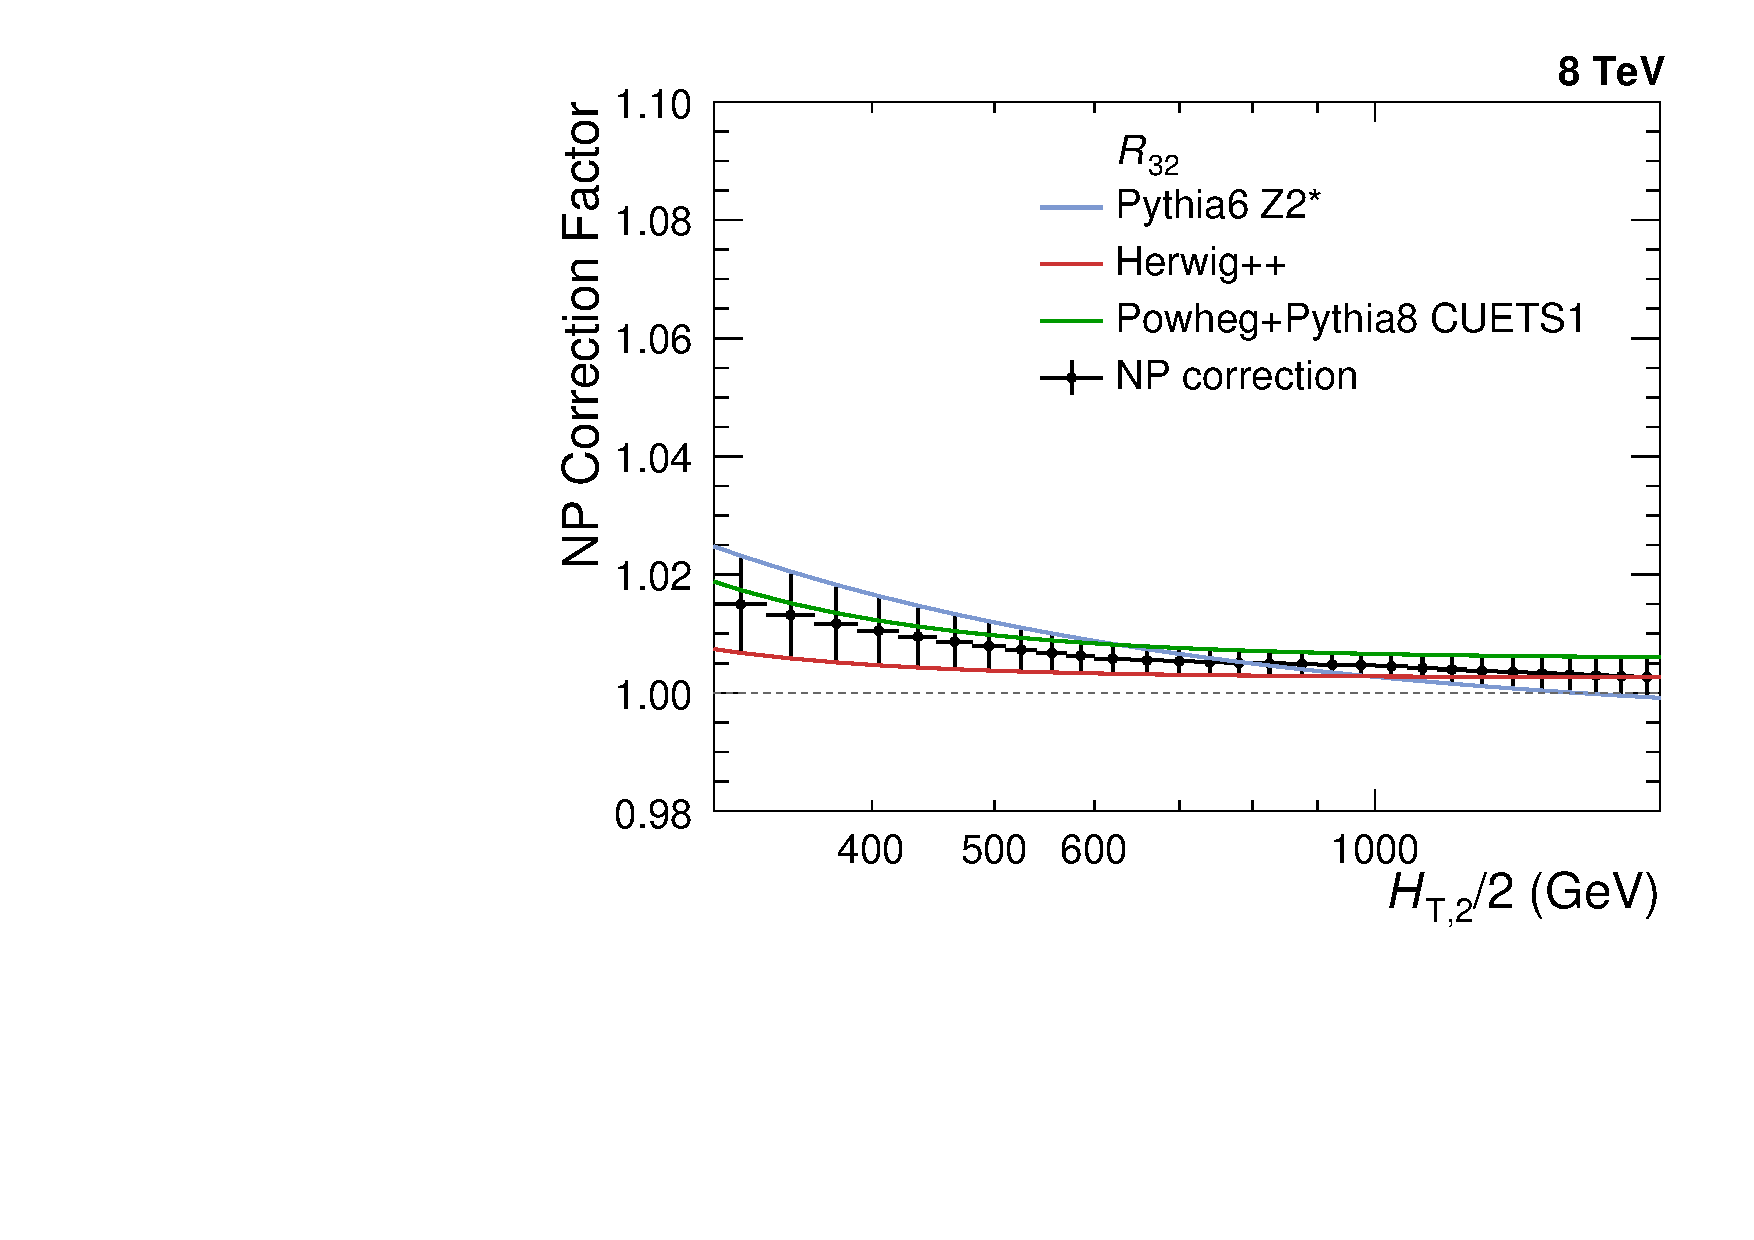
\includegraphics[width=0.5\textwidth]{Plots_PAS/Final_NP_Corr_Ratio_32.pdf}\hftwo
  \caption{Fits to the nonperturbative corrections obtained for
    inclusive 2-jet (top \cmsLeft) and 3-jet (top \cmsRight) event
    cross sections and their ratio \ratio (bottom) as a function of
    \httwo within $|y|<2.5$ for the three investigated MC event
    generators.}
  \label{fig:np_factors}
\end{figure}

The NP corrections are shown in Fig.~\ref{fig:np_factors} for the
inclusive 2-jet (top \cmsLeft) and 3-jet event cross sections (top
\cmsRight) as well for \ratio (bottom). They amount to $\approx$
4--5\% for inclusive 2-jet and 3-jet events and $\approx$ 1\% for
\ratio at \httwo $\approx$ 300\GeV and decrease for increasing
\httwo. The uncertainty assigned to the NP corrections is of the order
of 1--2\%. The non-perturbative effects are reduced in the cross
section ratio.

\begin{figure}[h]
  \hftwo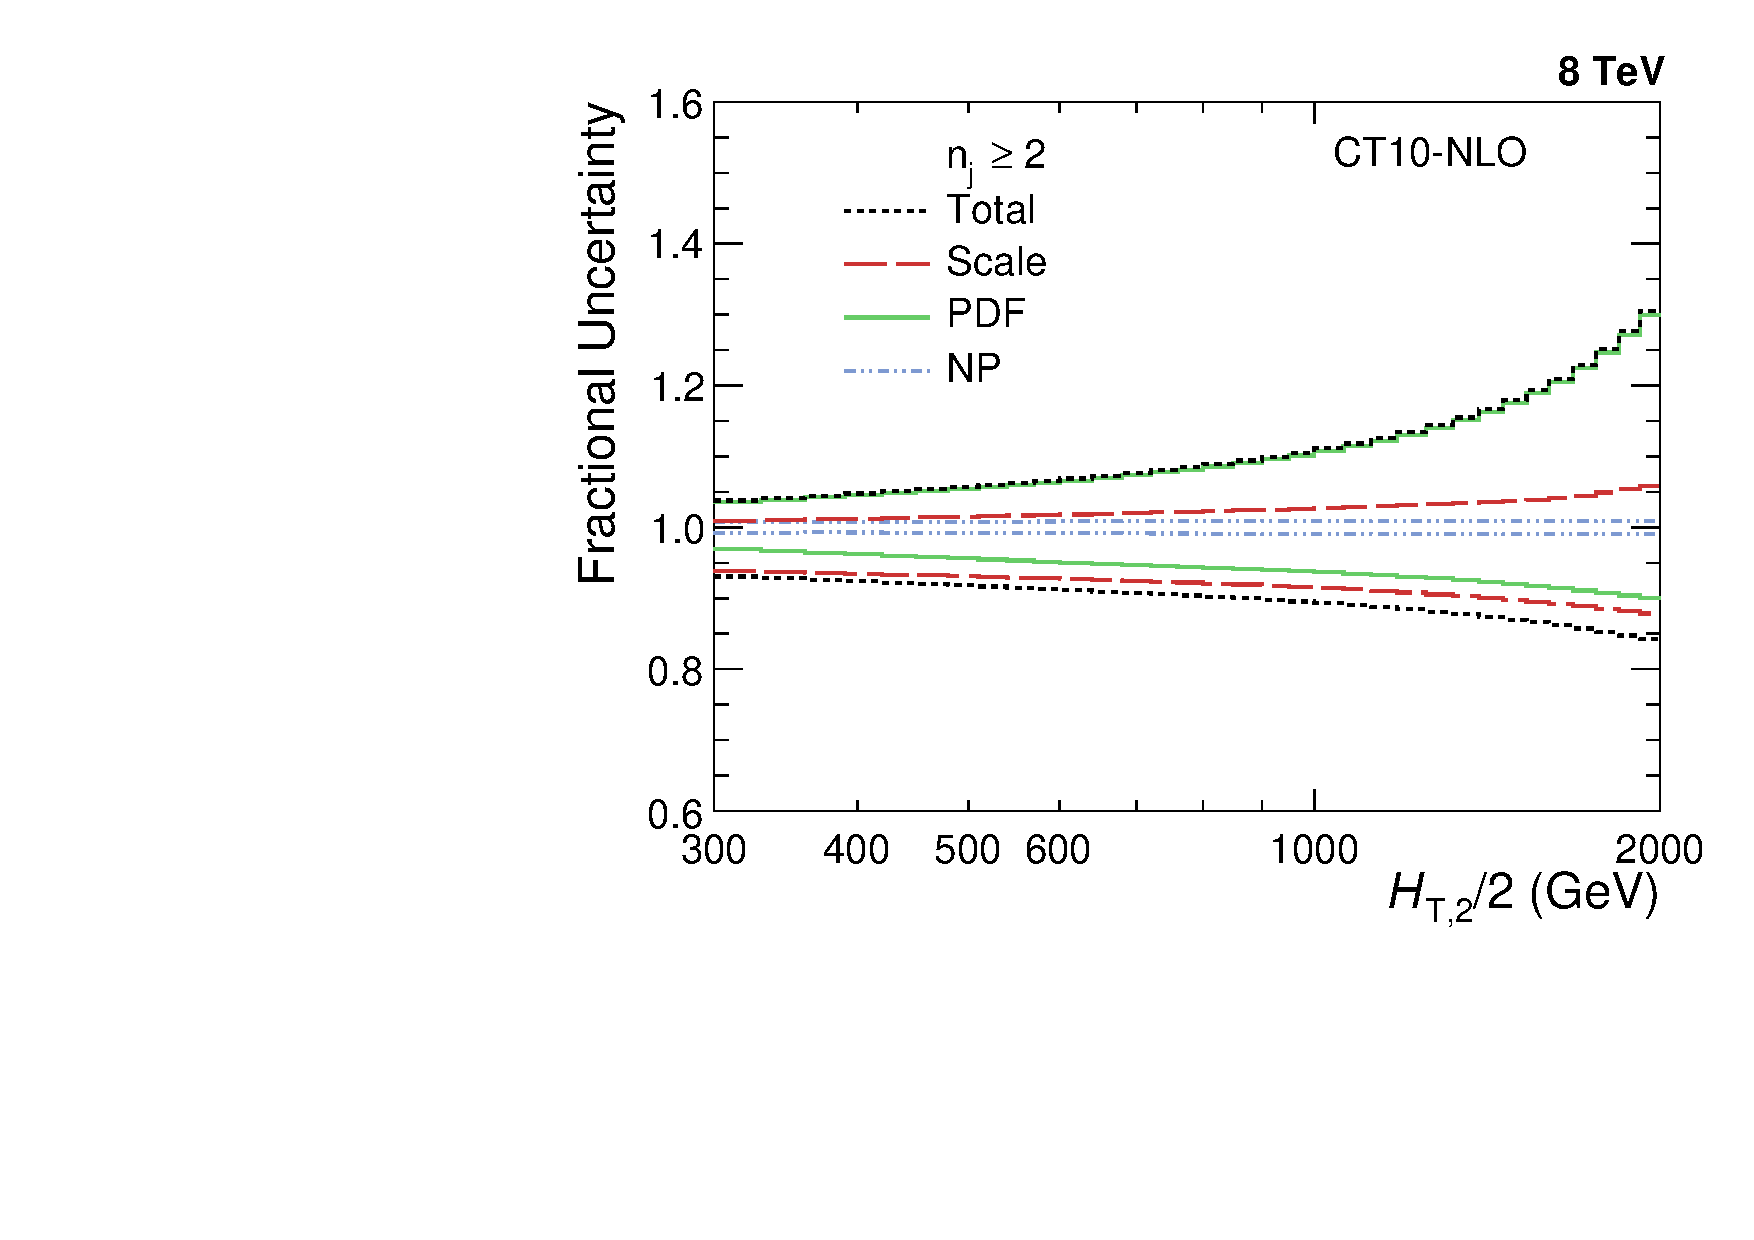
\includegraphics[width=0.5\textwidth]{Plots_PAS/Theory_Unc_2.pdf}\hftwo%
  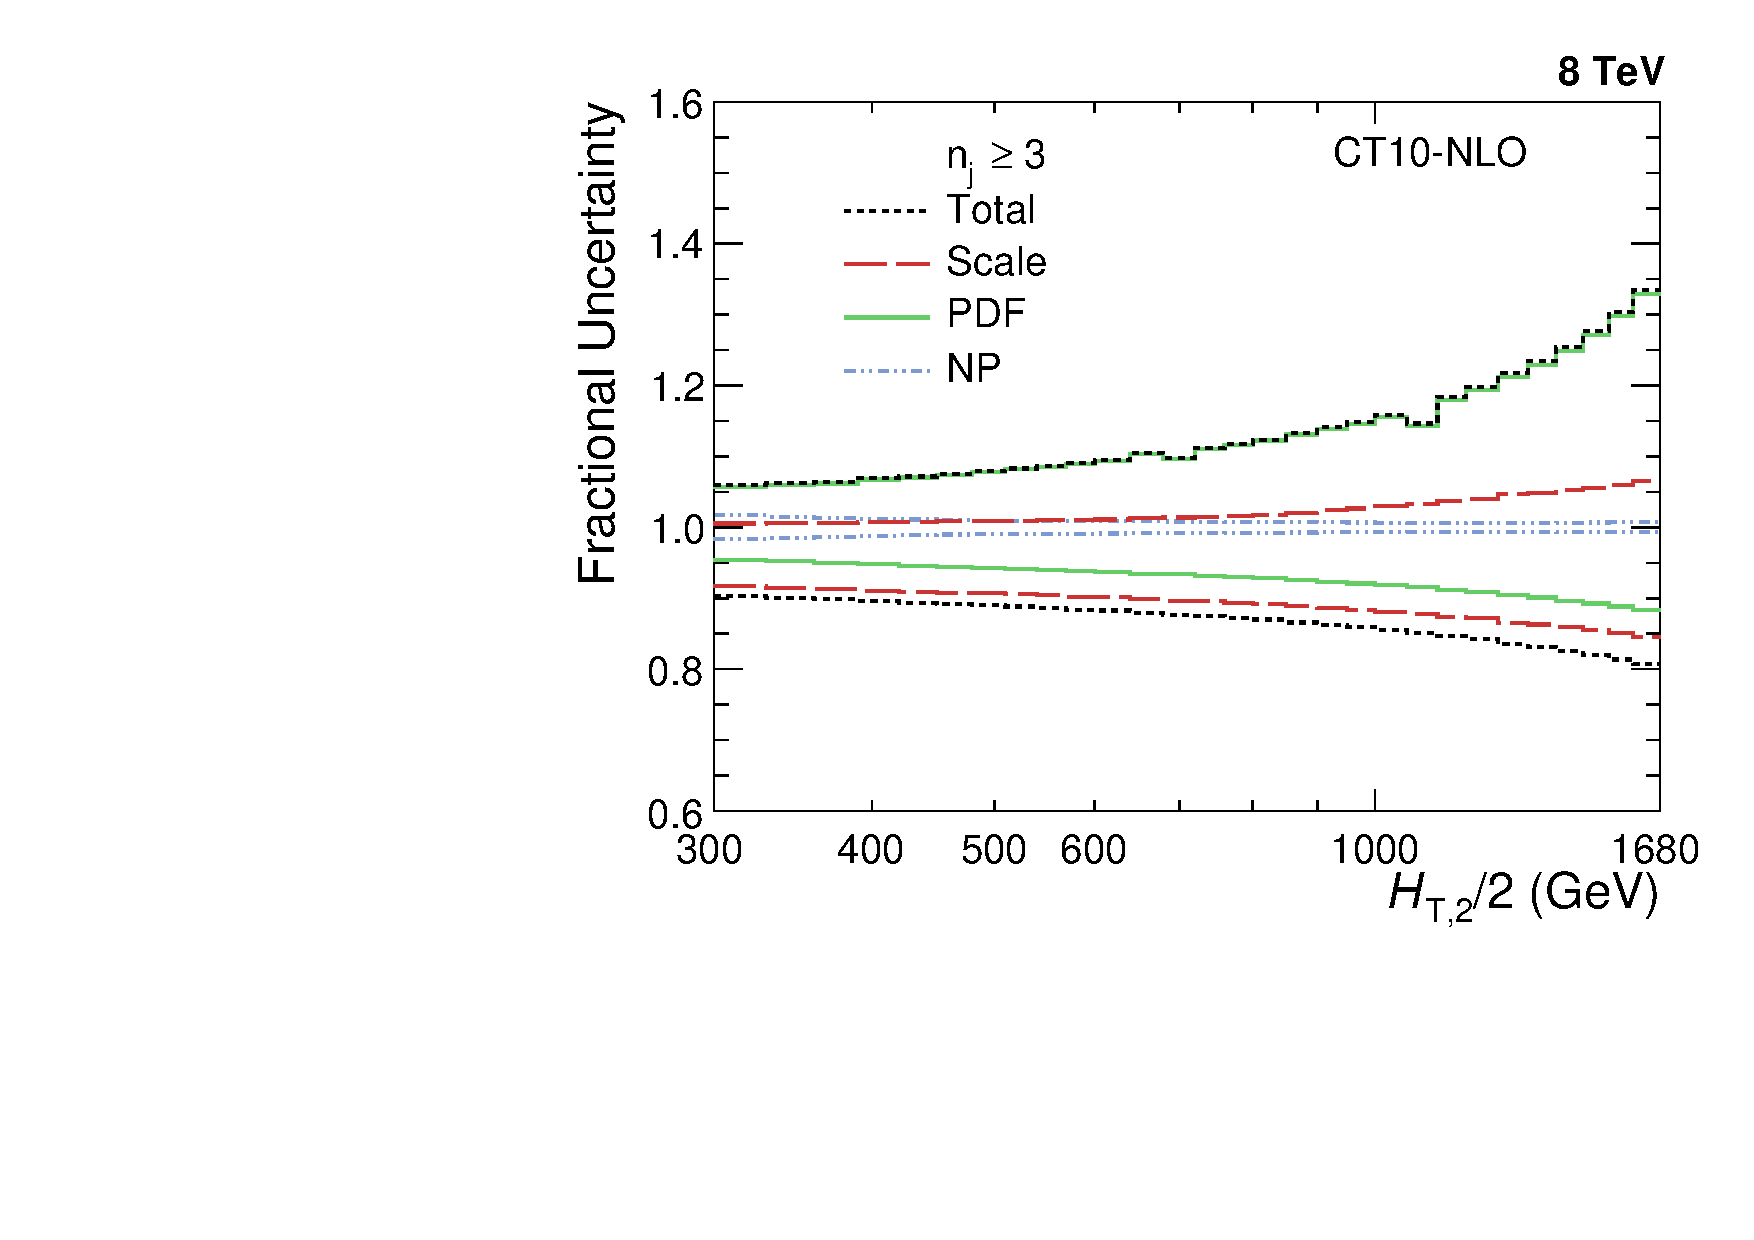
\includegraphics[width=0.5\textwidth]{Plots_PAS/Theory_Unc_3.pdf}\hftwo\\
  \hftwo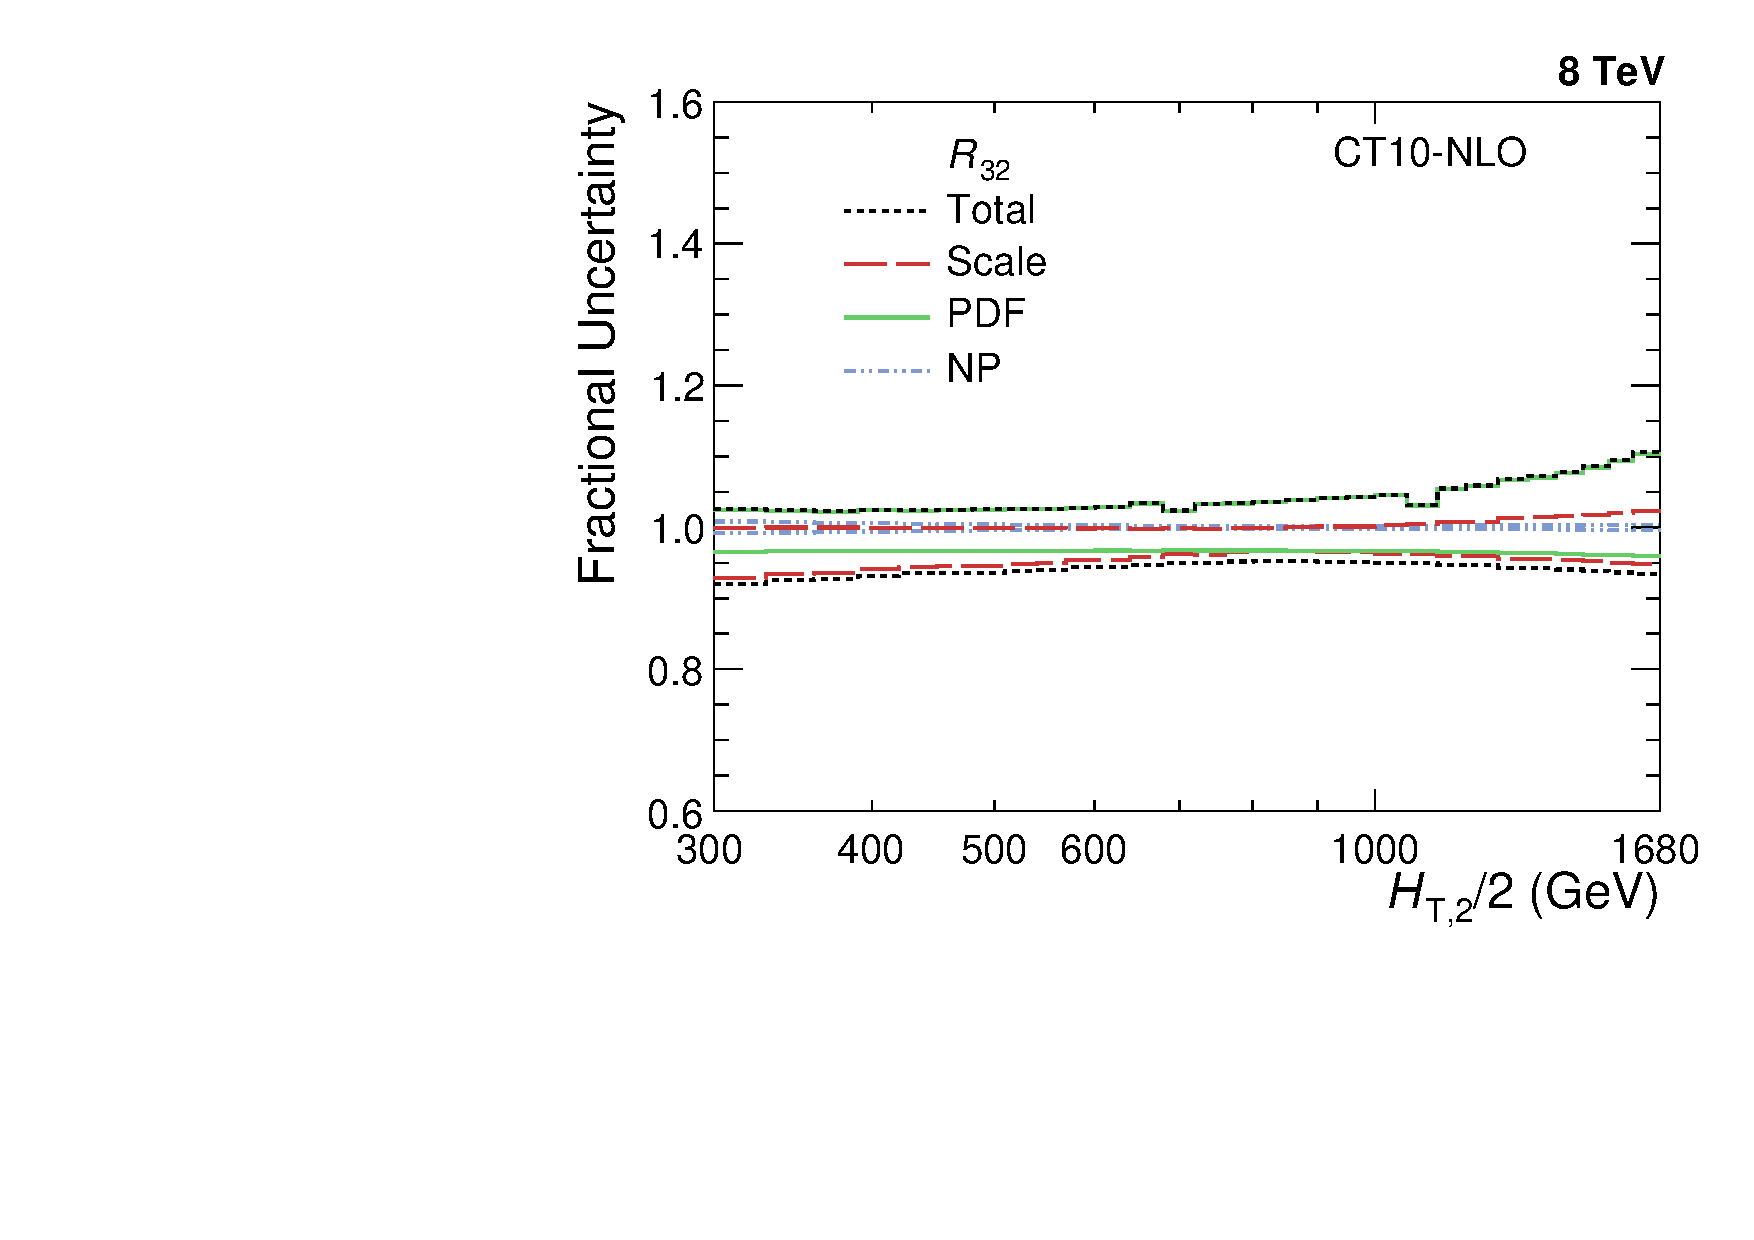
\includegraphics[width=0.5\textwidth]{Plots_PAS/Theory_Unc_Ratio_32.pdf}\hftwo
  \caption{Overview of theoretical uncertainties affecting the cross
    section prediction for inclusive 2-jet (top \cmsLeft) and 3-jet
    events (top \cmsRight) and their ratio \ratio (bottom), using the CT10 PDF set. The total uncertainty
    is calculated by adding in quadrature the individual sources of
    uncertainty. The statistical uncertainties of the NLO computations
    are too small to be visible and are not shown.}
  \label{fig:theory_unc}
\end{figure}

The total theoretical uncertainties are evaluated as the quadratic sum
of the scale, PDF, NP, and statistical
uncertainties. Figure~\ref{fig:theory_unc} presents an overview of the
theoretical uncertainties affecting the cross section prediction for
inclusive 2-jet (top \cmsLeft) and 3-jet events (top \cmsRight) and their ratio \ratio (bottom),
using the CT10 PDF set.
\end{comment}
